\documentclass{article}
\usepackage[utf8]{inputenc}
\usepackage{pgfplots}
\pgfplotsset{width=10cm,compat=1.9}
\usepackage{amsmath,amssymb,amsthm}
\usepackage{graphicx}
\usepackage{float}
\usepackage{blindtext}
\usepackage{hyperref}
\usepackage{verbatim}
\usepackage{gensymb}
\usepackage{enumerate}
\usepackage{xcolor}
\usepackage{graphicx}
\hypersetup{
    colorlinks=true,
    linkcolor=blue,
    filecolor=magenta,      
    urlcolor=cyan,
    pdftitle={Overleaf Example},
    pdfpagemode=FullScreen,
    }
\usepackage[slovene]{babel}

\setlength{\parindent}{0pt}
\setlength{\parskip}{4pt}

\newcounter{example}[section]
\newenvironment{example}[1][]{\refstepcounter{example}\par\medskip
   \noindent \textbf{Naloga~\theexample. #1} \rmfamily}{\medskip}

\newtheorem*{zgled}{Zgled}

\title{Kotne funkcije}
\author{Bor Bregant}
\date{\vspace{-5ex}}

\begin{document}

\maketitle

\begin{figure}[H]
    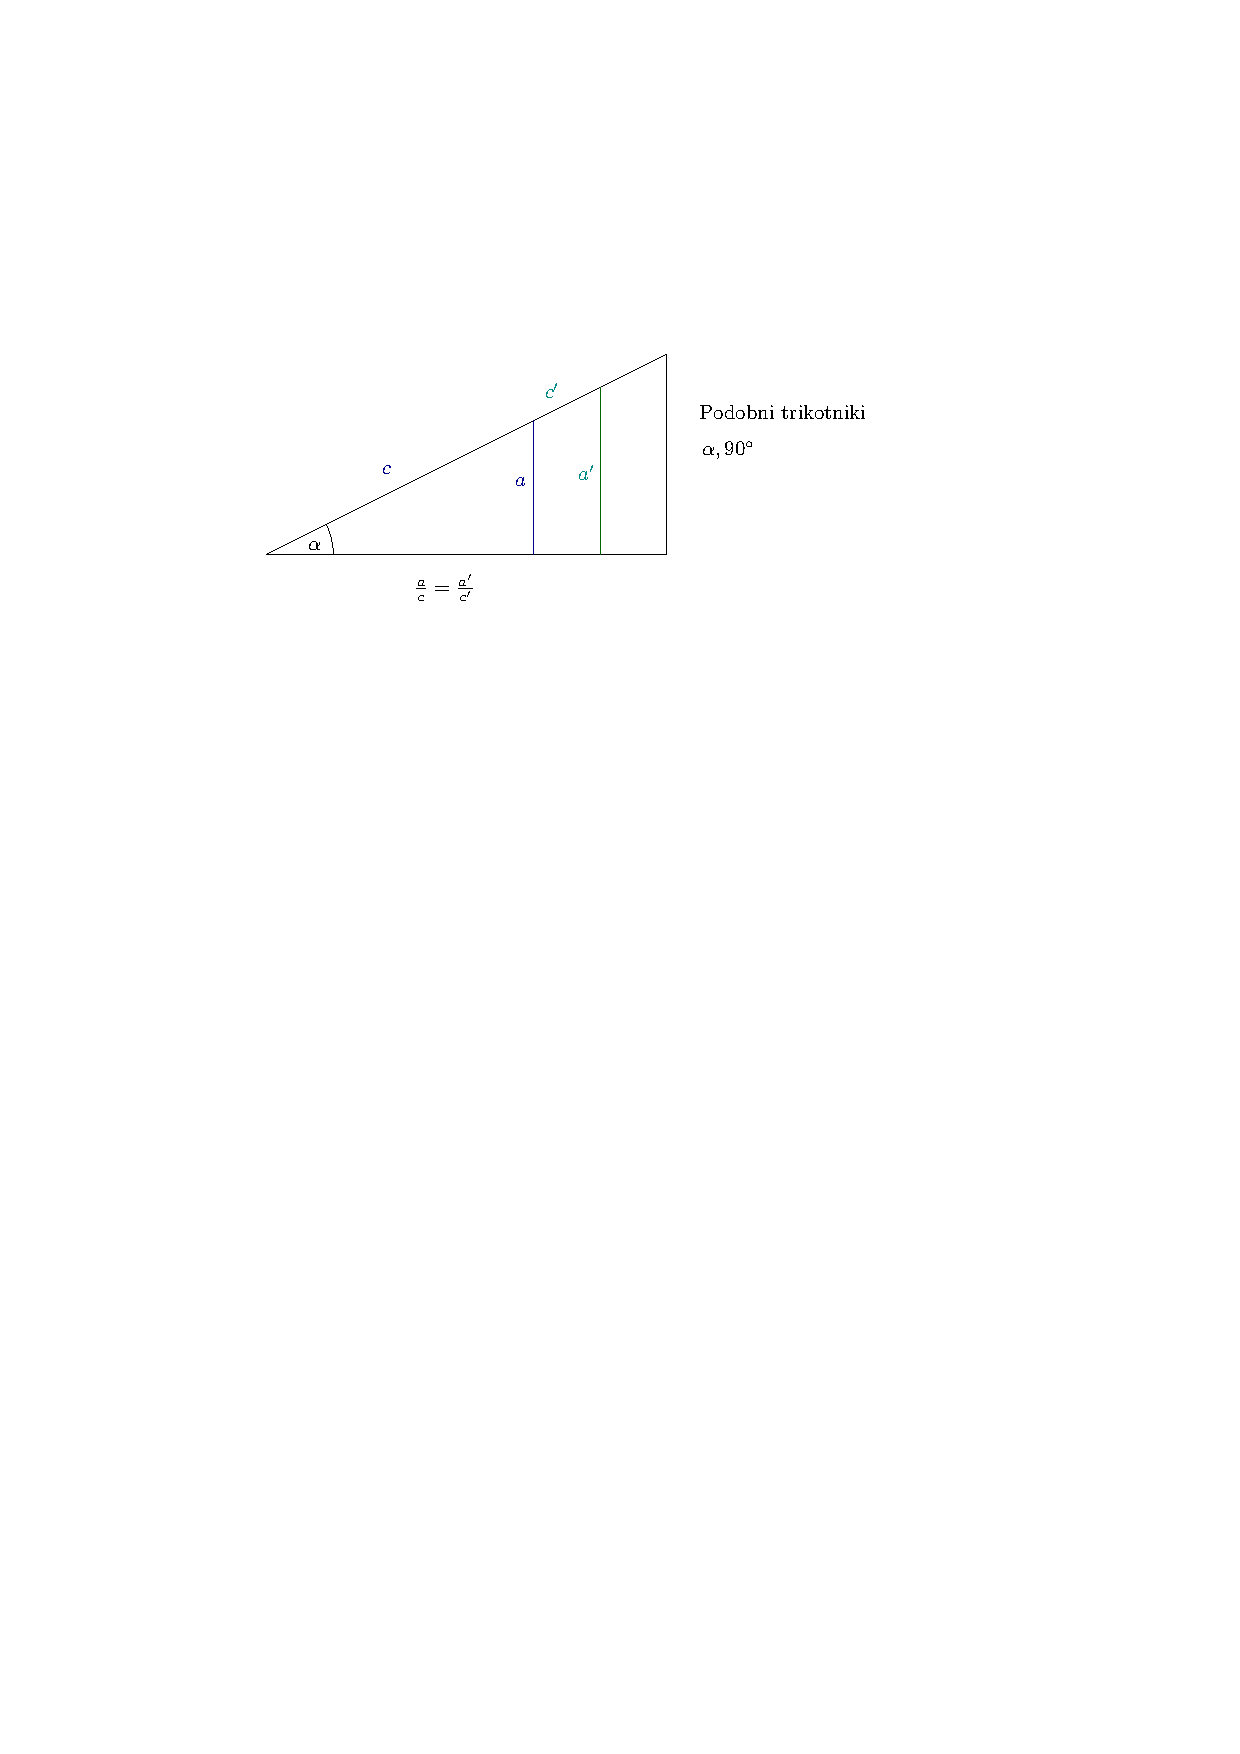
\includegraphics[width=0.7\textwidth]{kotne_funkcije.pdf}
    \centering
\end{figure}

\begin{enumerate}[i]
    \item $\sin{\alpha}=\frac{\text{nepriležna kateta}}{\text{hipotenuza}}=\frac{a}{c}$
    \item $\cos{\alpha}=\frac{\text{priležna kateta}}{\text{hipotenuza}}=\frac{b}{c}$
    \item $\tan{\alpha}=\frac{\text{nepriležna kateta}}{\text{priležna kateta}}=\frac{a}{b}$
    \item $\cot{\alpha}=\frac{\text{priležna kateta}}{\text{nepriležna kateta}}=\frac{b}{a}$
\end{enumerate}

Kotne funkcije so odvisne od kota $\alpha$

\section{Zveze med kotnimi funkcijami}

Izpeljave z oznakami stranic razen zadnji dve

\begin{align*}
    \tan \alpha &= \frac{\sin\alpha}{\cos\alpha}\\
    \cot\alpha &= \frac{\cos\alpha}{\sin\alpha}\\
    \tan \alpha \cdot \cot\alpha &= 1\\
    \sin^2\alpha +\cos^2\alpha &= 1\\
    1+\tan^2\alpha &= \frac{1}{\cos^2\alpha}\\
    1+\cot^2\alpha &= \frac{1}{\sin^2\alpha}
\end{align*}

\begin{zgled}
    Nariši ostri kot $x$, če je $\sin x =\frac{2}{5}$.
\end{zgled}

\begin{zgled}
    Poenostavi izraz $\tan x -\sin x : \left(\cos x - \cos^{-1} x \right)$
\end{zgled}

\begin{example}
    DN Naredi si plonk listek vseh pomembnih formul in zvez, 185, 188, 189
\end{example}

%\begin{zgled} ta je iz DN
%    Poenostavi $\frac{\cos x}{1-\sin x}-\frac{\cos x}{1+\sin x}$.
%\end{zgled}

1 radian je kot, ki pripada loku, dolgemu natanko polmer krožnice.

\begin{figure}[H]
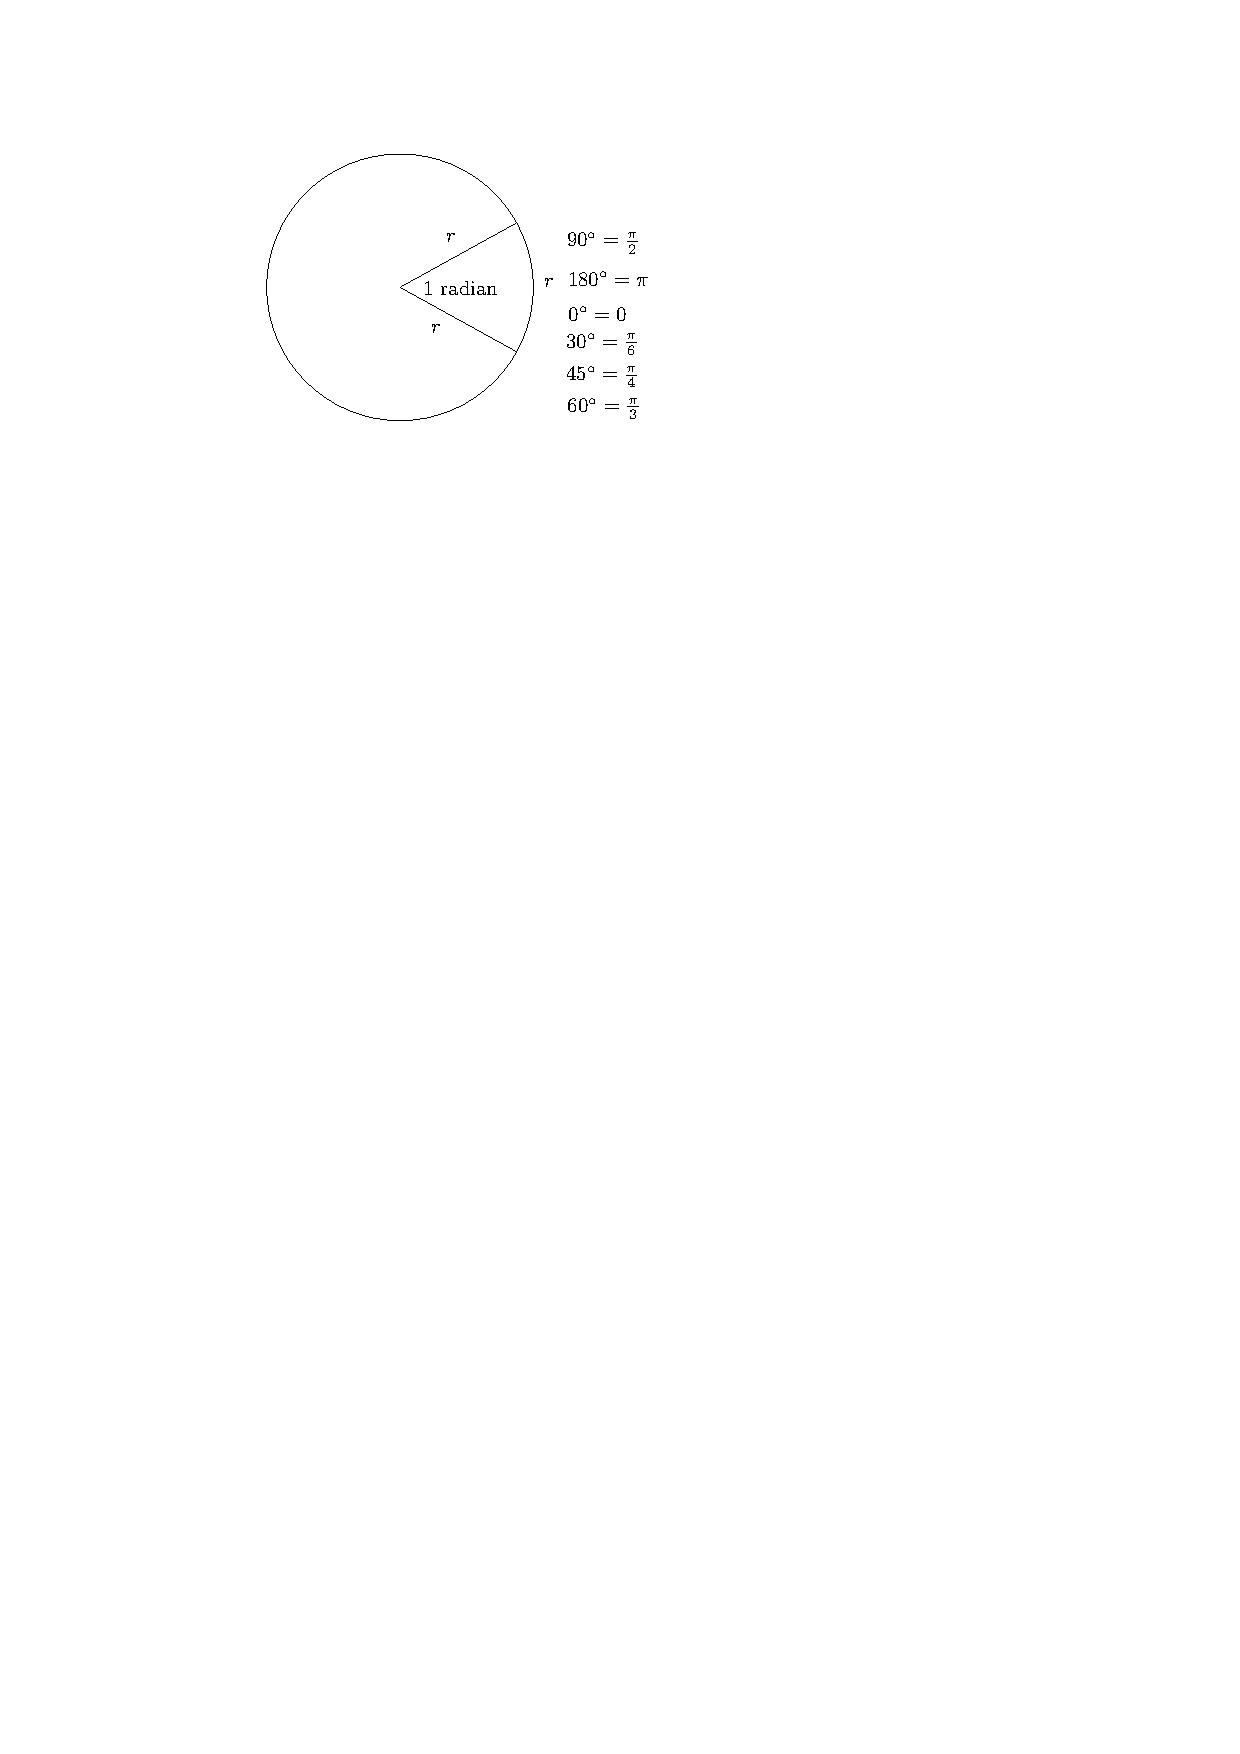
\includegraphics[width=0.4\textwidth]{trigonometrija.radiani.pdf}
\centering
\end{figure}

%\begin{figure}[H]
%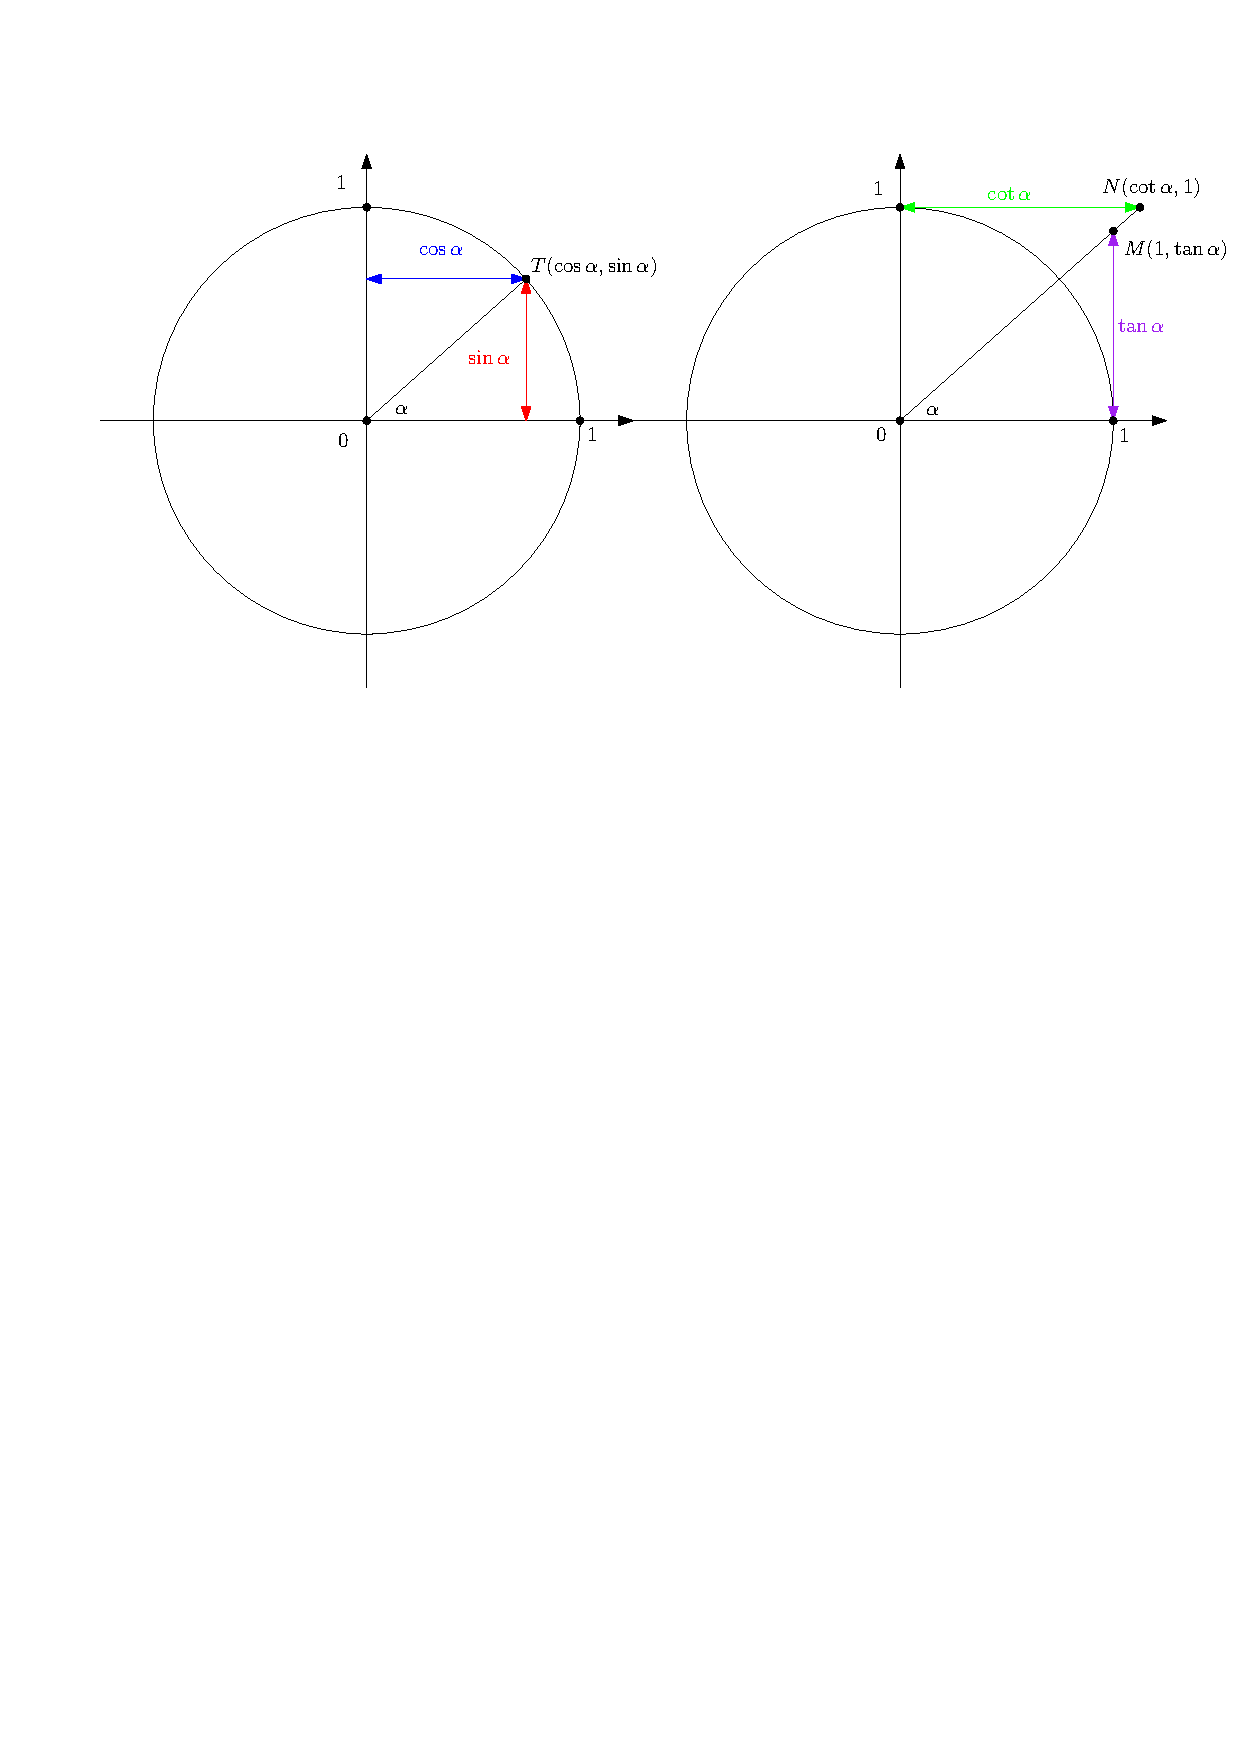
\includegraphics[width=0.8\textwidth]{trigonometrija.enotska.pdf}
%\centering
%\end{figure}

\begin{tabular*}{\linewidth}[b]{*{6}{|c @{\extracolsep\fill}}|}
\hline  Kot $\angle^\circ \rightarrow$   &0$^\circ$& 30$^\circ$ & 45$^\circ$ & 60$^\circ$ & 90$^\circ$
\\ $\downarrow$ Funkcija $\angle ^\circ$ &  &  &  &  & \\ 
\hline $\sin \theta$ & 0 & $\frac{1}{2}$ &$\frac{\sqrt{2}}{2}$ & $\frac{\sqrt{3}}{2}$& 1\\[15pt]
\hline $\cos \theta$ & 1 & $\frac{\sqrt{3}}{2}$ &$\frac{\sqrt{2}}{2}$ & $\frac{1}{2}$& 0\\ 
\hline $\tan \theta$ & 0 & $\frac{\sqrt{3}}{3}$ &1  & $\sqrt{3}$ & ND\\
\hline
$\cot \theta$ & ND & $\sqrt{3}$ &1 & $\frac{\sqrt{3}}{3}$ & 0 \\ \hline
\end{tabular*}

Izpeljava $\sin 60^\circ$ iz enakostraničnega trikotnika z višino (iz Pitagorovega). $30^\circ$ vidimo v istem trikotniku zgoraj. $45^\circ$ vidimo v diagonali kvadrata.

\begin{figure}[H]
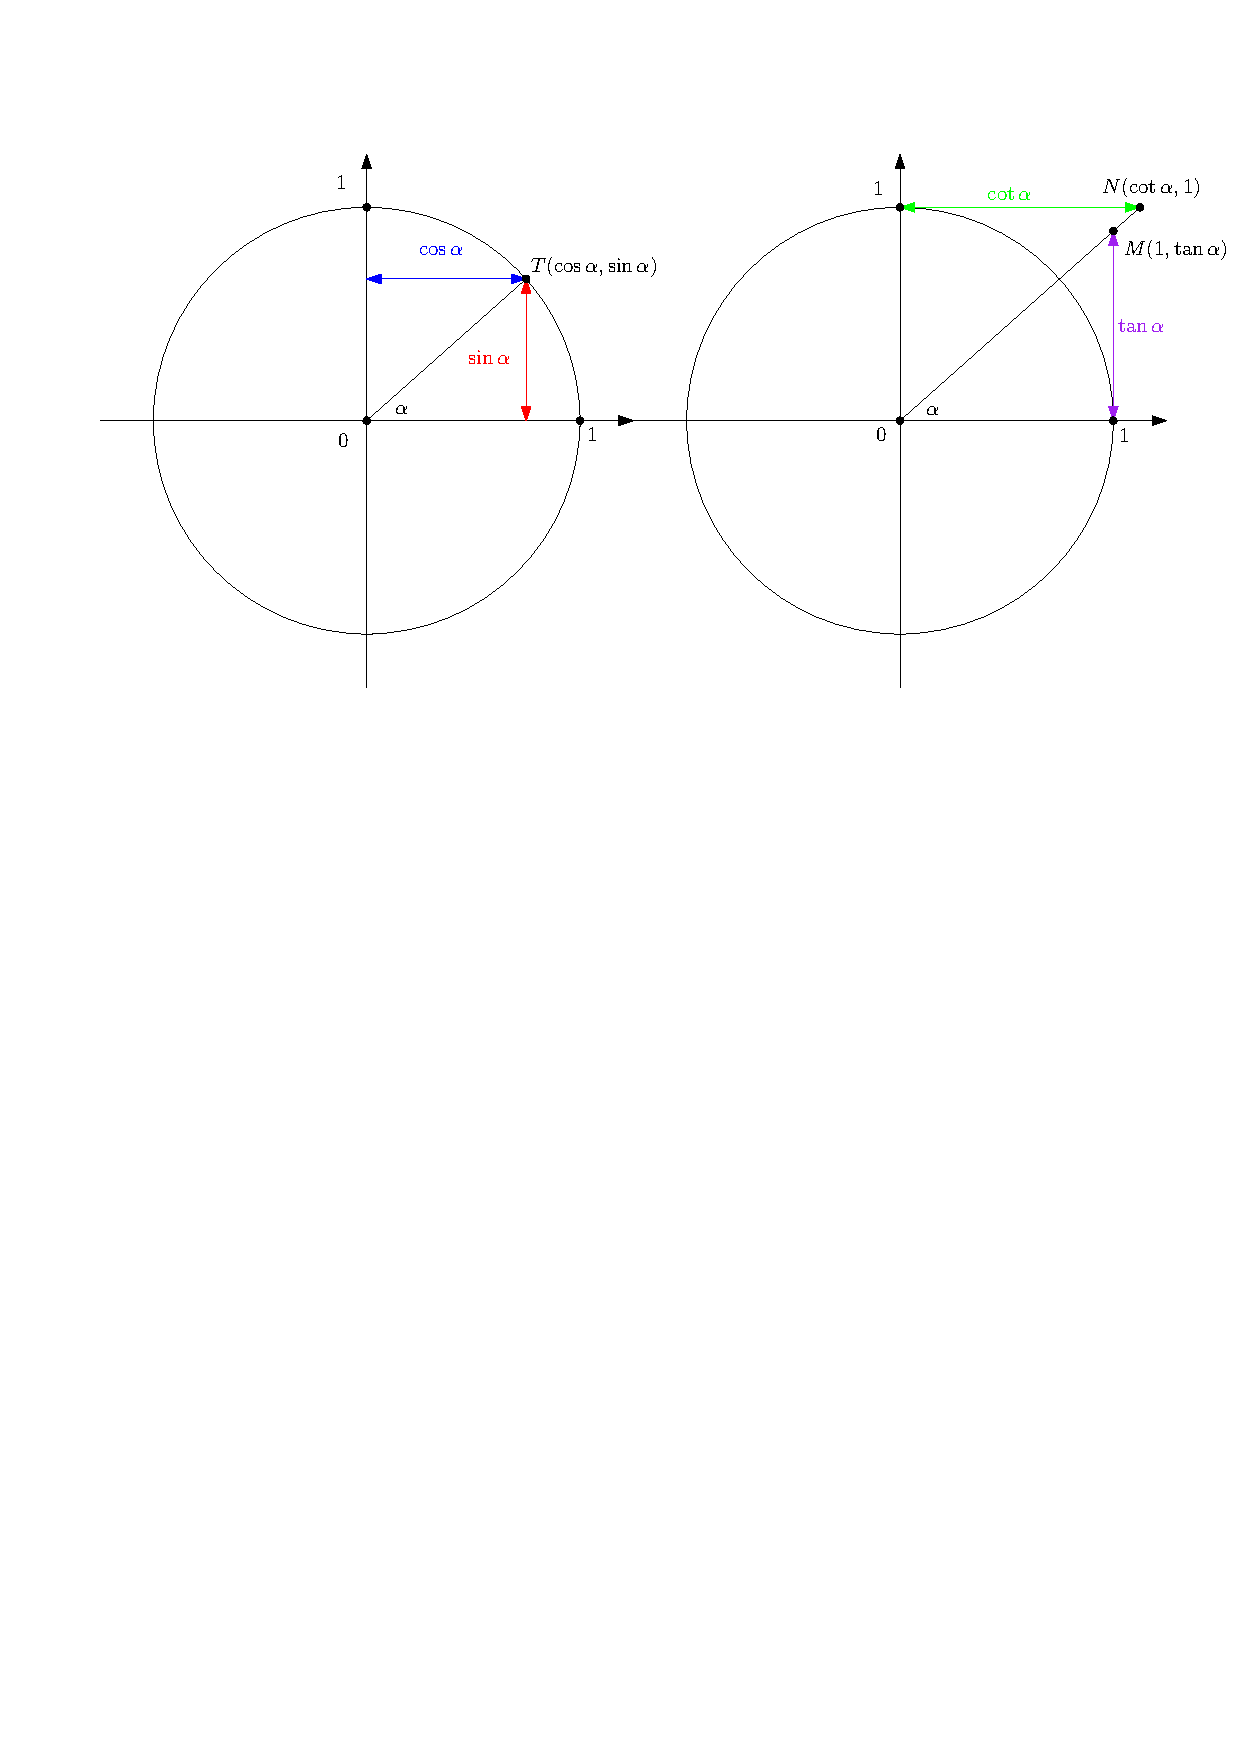
\includegraphics[width=0.8\textwidth]{trigonometrija.enotska.pdf}
\centering
\end{figure}

\begin{example}
    DN Nauči se tabelo
\end{example}

\end{document}